\documentclass[12pt,letterpaper]{article}
\usepackage[utf8]{inputenc}
\usepackage[spanish]{babel}
\usepackage{amsmath}
\usepackage{subcaption}
\usepackage{amsfonts}
 \usepackage{hyperref}
\usepackage{amssymb}
\usepackage{listings}
\usepackage{graphicx}
\usepackage[left=2cm,right=2cm,top=2cm,bottom=2cm]{geometry}
\setlength{\parskip}{3mm}
\title{\textsc{Ajuste de distribución}}
\author{\textsc{Fabiola Vázquez}}

\setlength{\parindent}{0cm}

\begin{document}
\maketitle

\hrule
\section{Introducción}
En un trabajo anterior \cite{fabiola} se realizó un estudio de la novela \textit{Alice's Adventures in Wonderland} \cite{alice}, donde se obtuvieron las palabras y las letras más frecuentes que aparecen en el libro. El objetivo de este estudio, que se realiza con el software estadístico R versión 4.0.2 \cite{R} en el IDE \textbf{R Studio} \cite{rstudio}, es estudiar las distribuciones de algunos de estos elementos del texto.

\section{Análisis}
Se calcula el largo de las oraciones en el texto y se realiza un histograma con estos datos, mismo que se puede ver en la figura \ref{historaciones}. Por nuestro conocimiento de distribuciones de probabilidad discretas, suponemos que el largo de las oraciones sigue una distribución geométrica. Con el uso de la función \texttt{fitdist} de la librería \texttt{fitdistrplus} se ajustan los datos a la distribución geométrica, obteniendo un parámetro \texttt{p=0.046}. Se generaron números pseudoaleatorios con esta distribución, tantos como oraciones en el texto, haciendo uso de \texttt{rgeom}. Un histograma de estos números se muestra en la figura \ref{historacionesrandom}.  La figura \ref{oraciones} muestra ambos histogramas lado a lado.

\begin{figure}
 	\centering 
 	\begin{subfigure}[b]{0.45\linewidth}
 		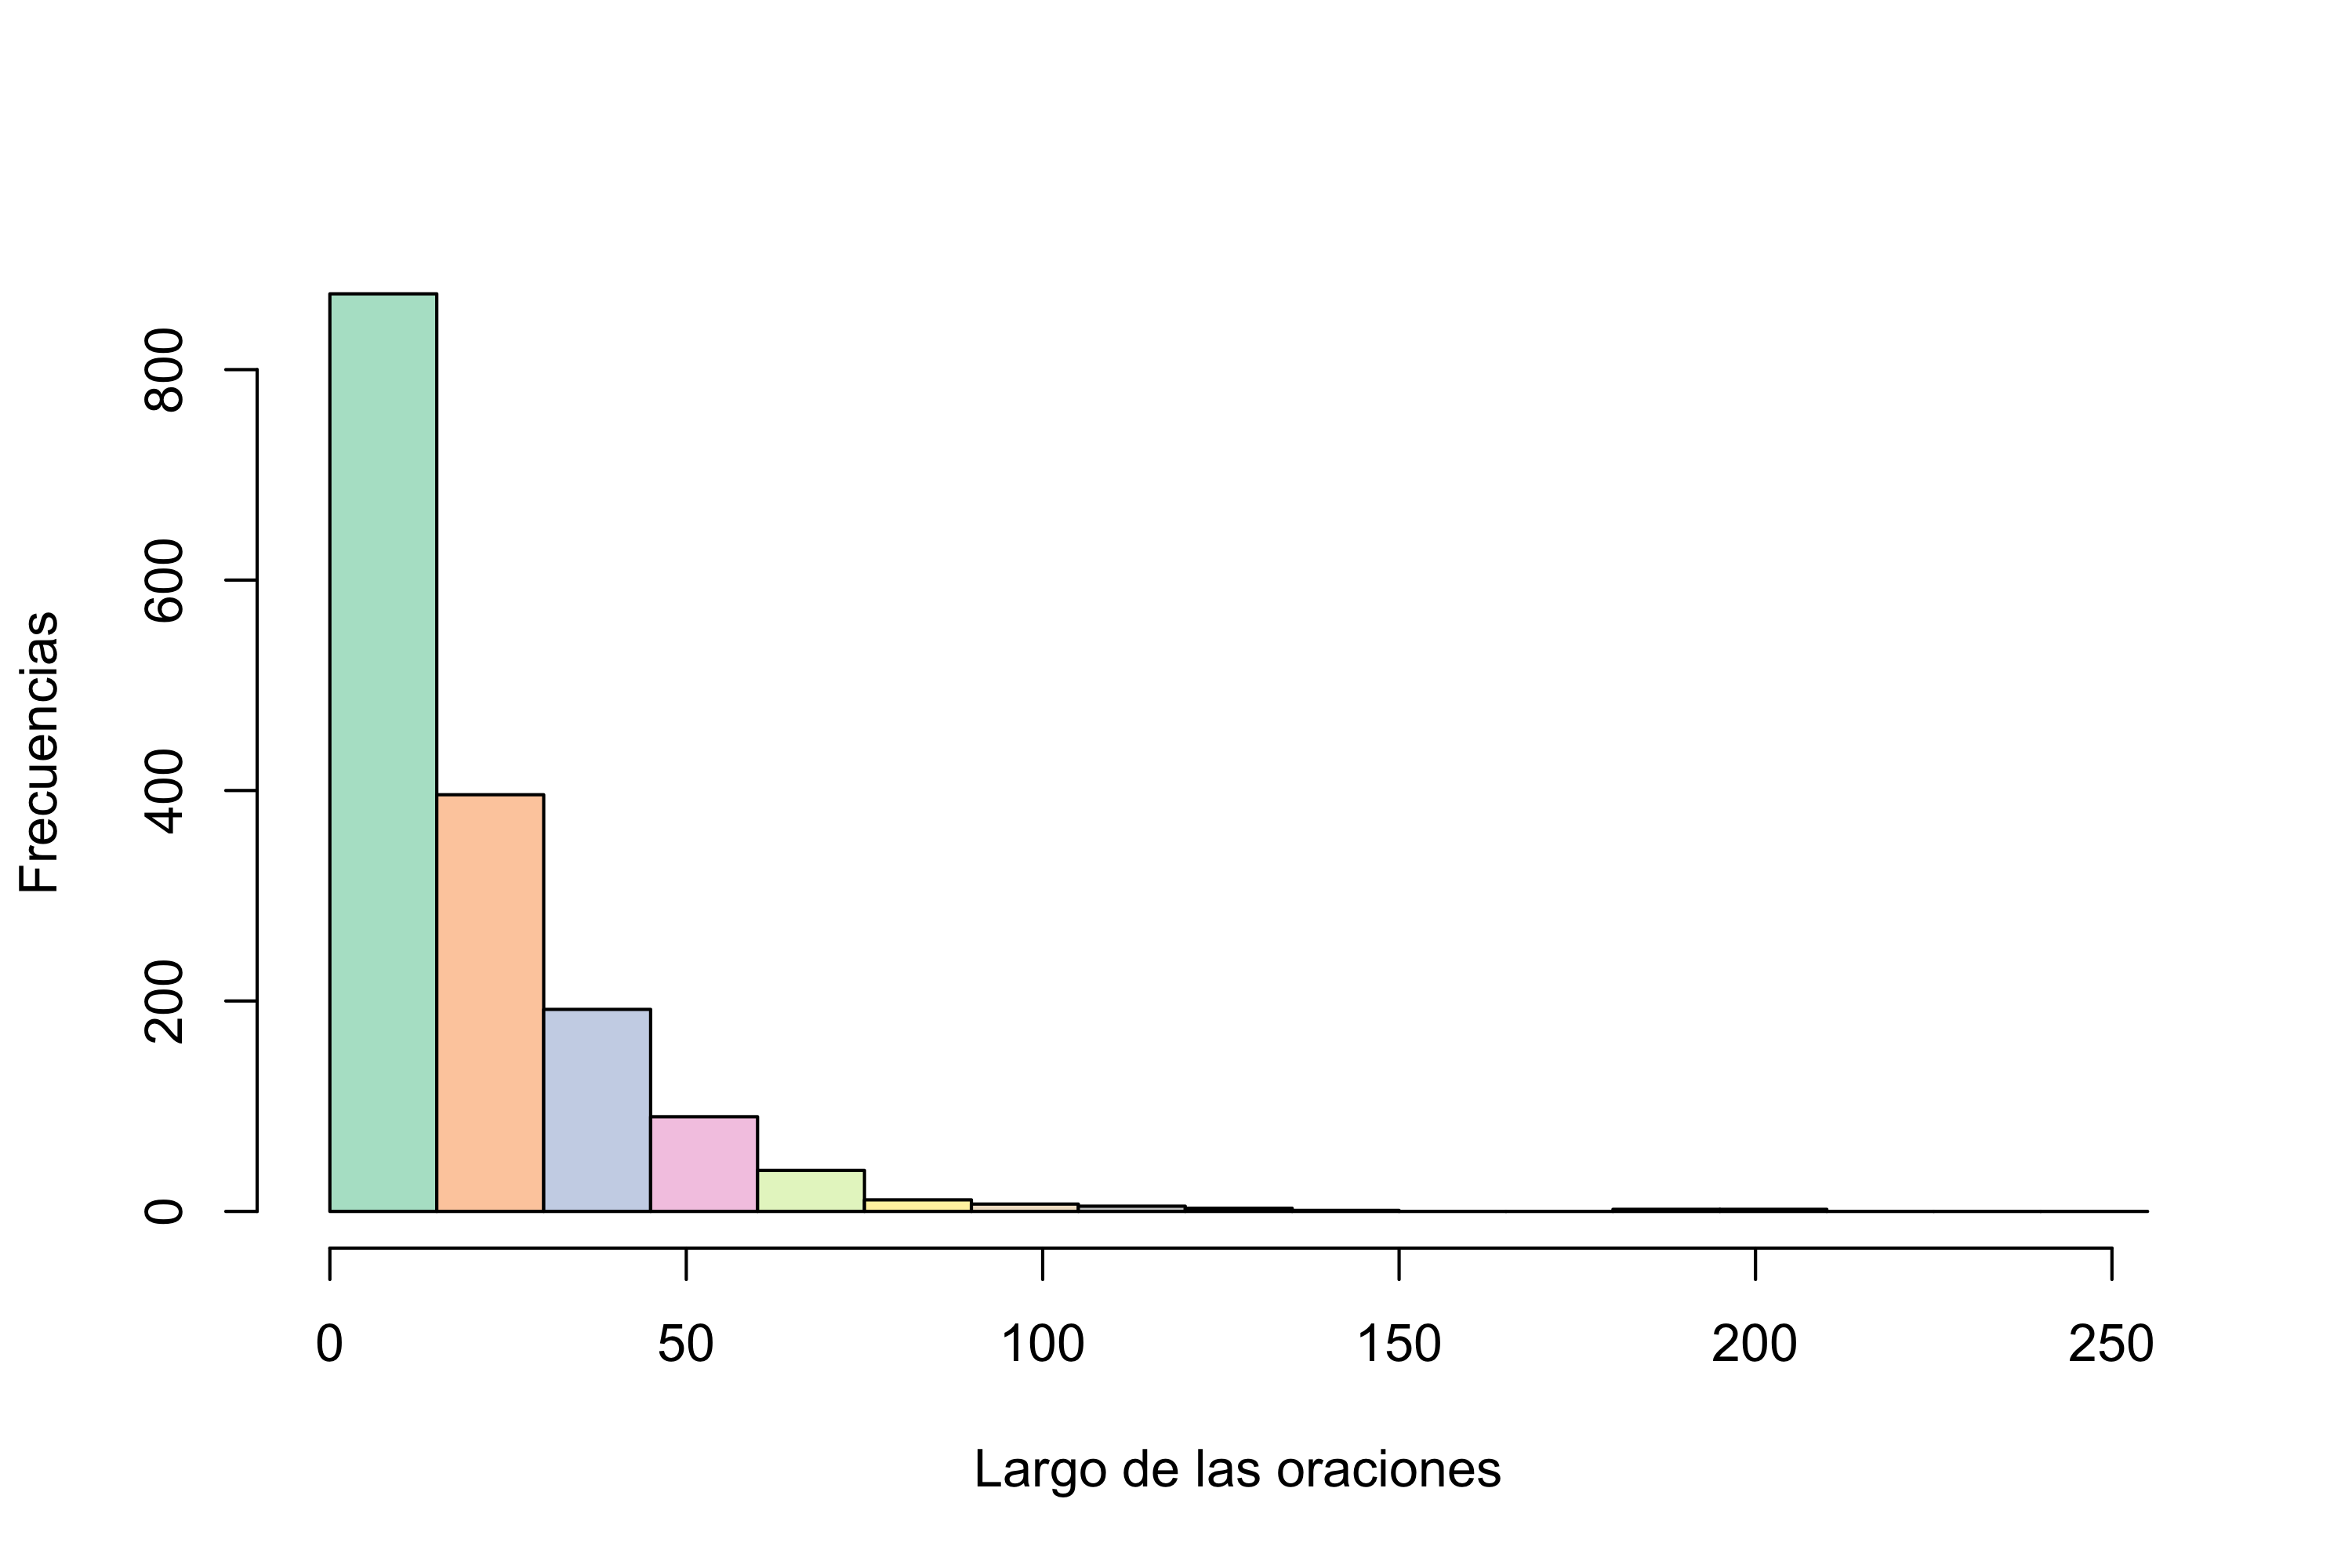
\includegraphics[width=\linewidth]{Largo_oraciones.png} 		
 		\caption{Largo de las oraciones.}
 		 		\label{historaciones}
 	\end{subfigure}
 	\begin{subfigure}[b]{0.45\linewidth}
 		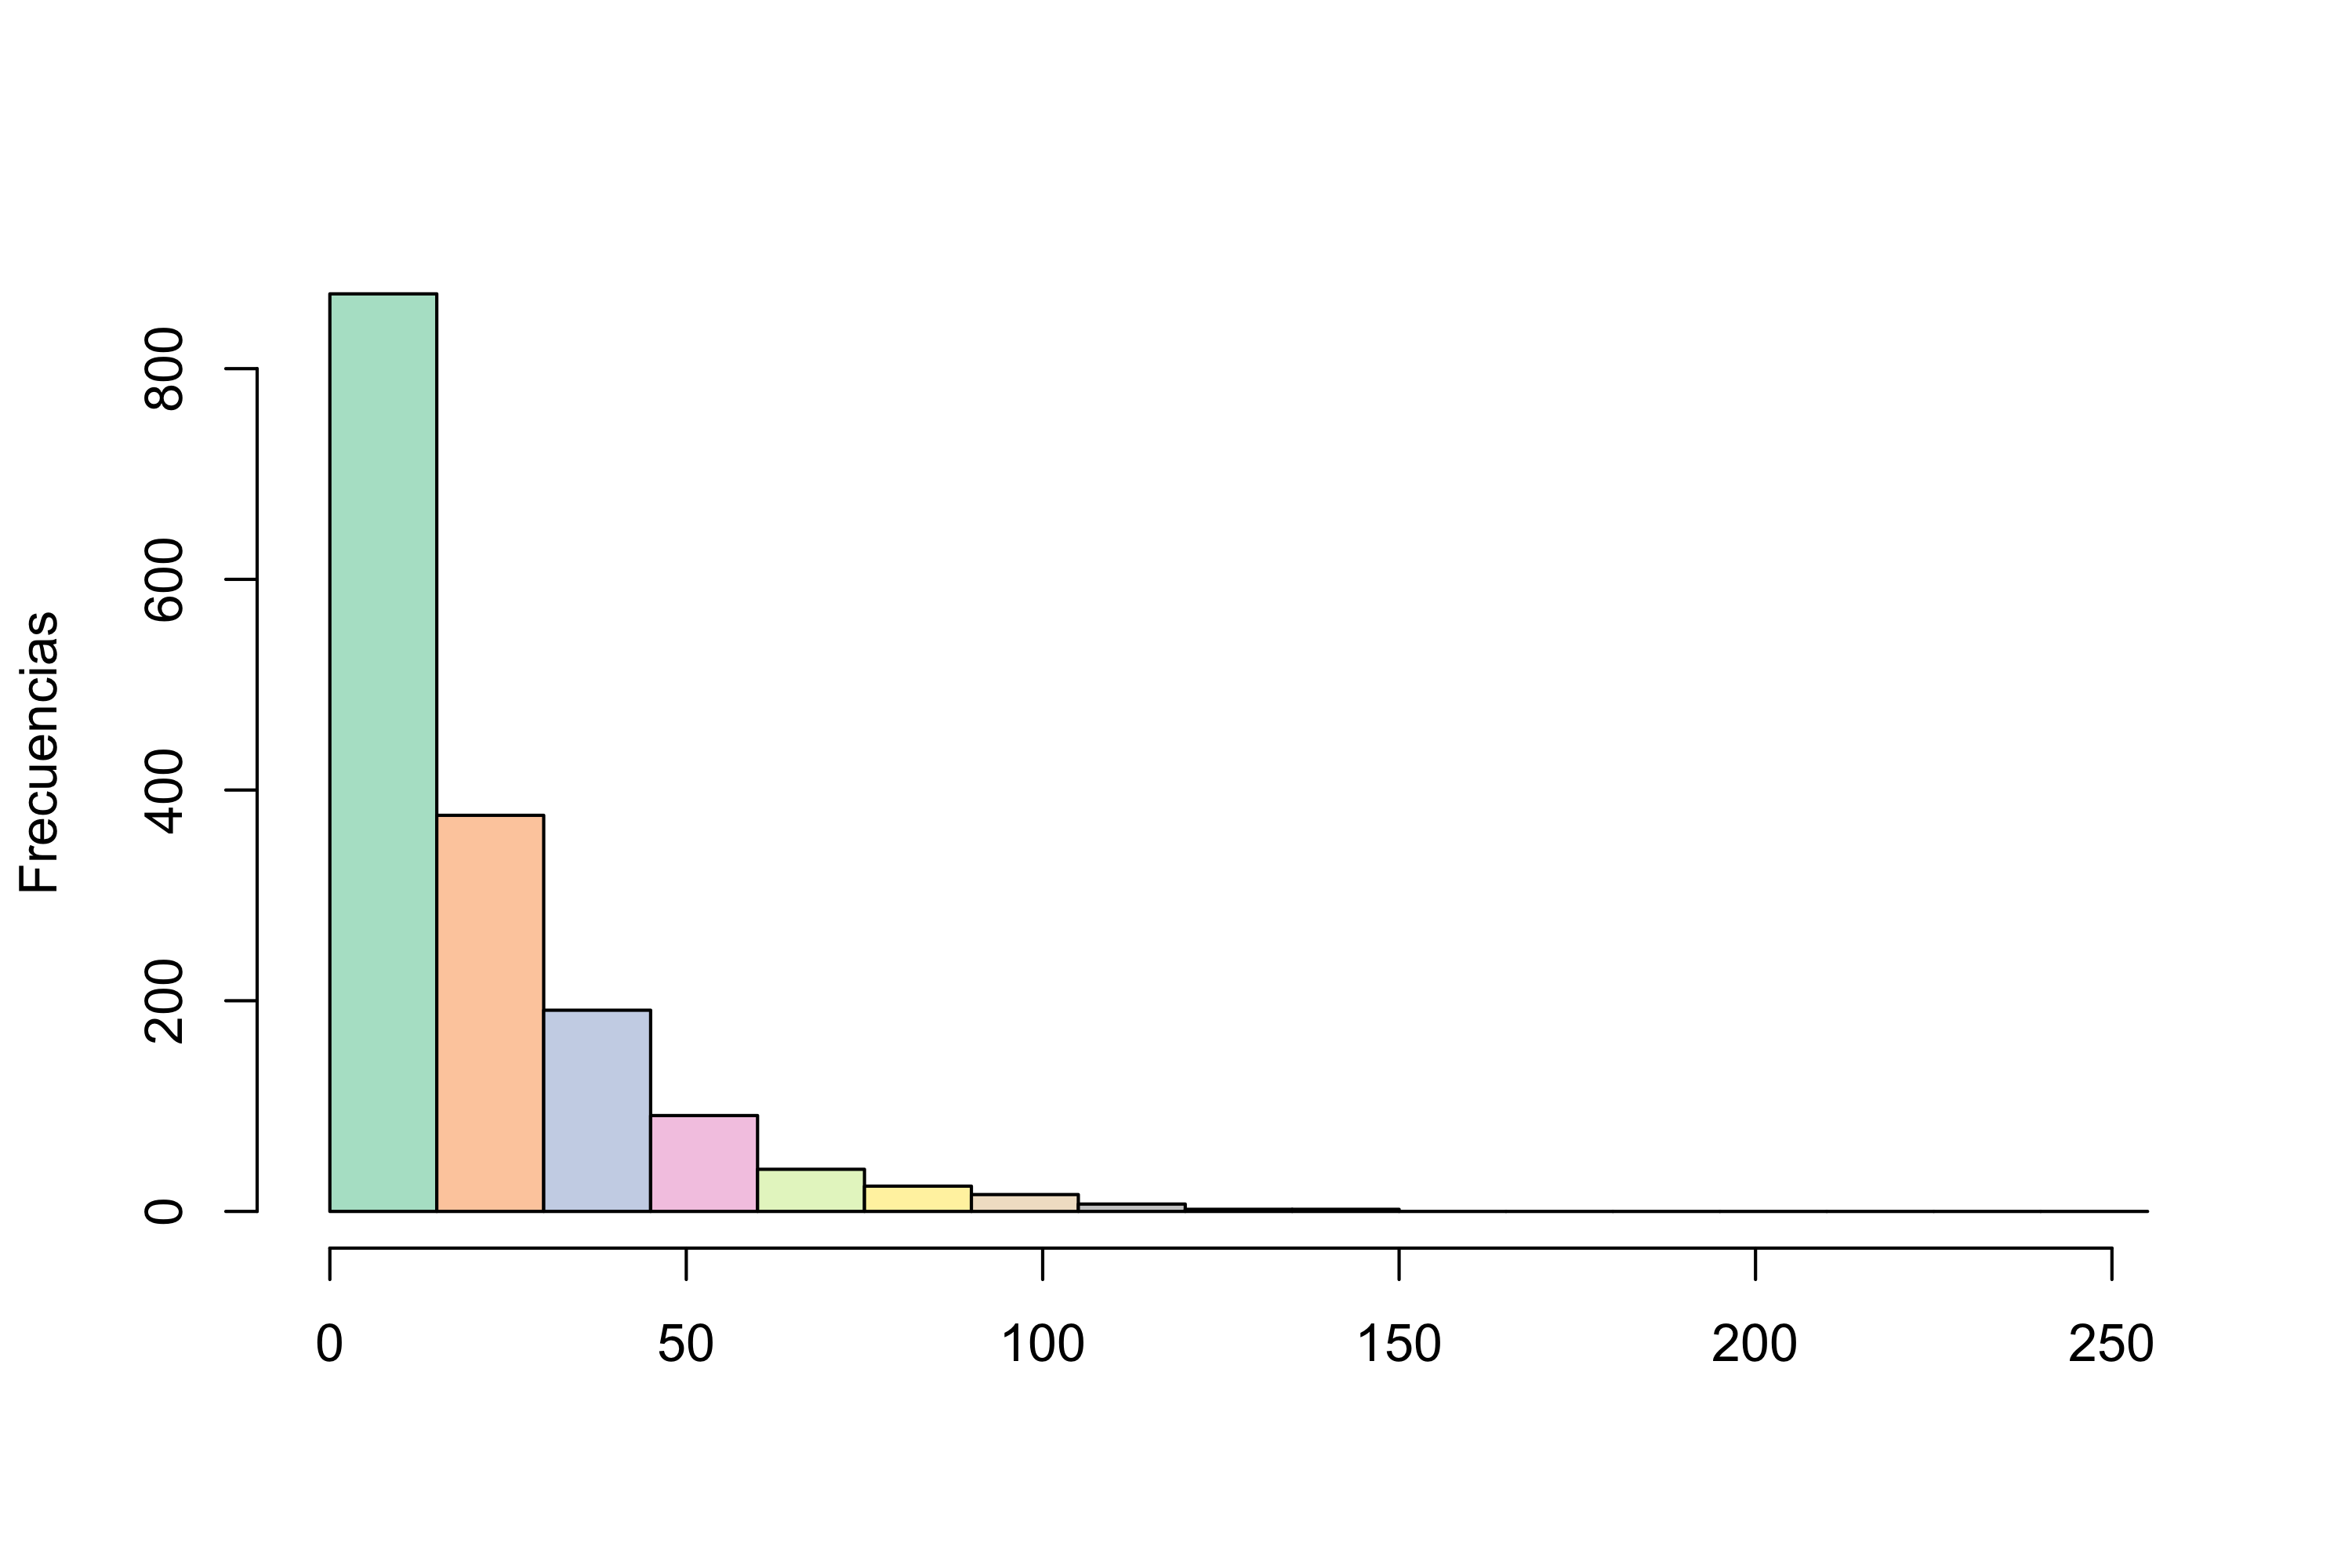
\includegraphics[width=\linewidth]{Largo_oraciones_distribucion.png} 		
 		\caption{Números pseudoaleatorios.}
 		\label{historacionesrandom}
 	\end{subfigure}

 	 	\caption{Distribución del largo de oraciones del libro.} 
 	 		\label{oraciones}
\end{figure}

Siguiendo el mismo procedimiento para el largo de los párrafos, se concluye que los datos se ajustan a una distribución geométrica con parámetro \texttt{p=0.028}. En la figura \ref{largoparrafos} se muestra el histograma de las longitudes de los párrafos del libro y el histograma de números pseudoaleatorios generados con distribución geométrica.

Después, se procede a buscar la distribución de la palabra \textit{Alice} en el texto. Para esto, se modela como un experimento Bernoulli, considerando como un éxito la aparición de la palabra \textit{Alice} y un fracaso cualquier otra palabra. Se obtuvo la cantidad de palabras que ocurrían entre cada aparición de la palabra \textit{Alice}, cuyo histograma se muestra en la figura \ref{alice}. Se obtiene que en promedio hay aproximadamente 66 palabras entre las apariciones de \textit{Alice}. Esto representa el promedio de fracasos antes de un éxito en una secuencia de experimentos Bernoulli, por lo que debe de seguir una distribución geométrica. Se sabe que esta distribución con parámetro $p$ tiene media $\frac{1-p}{p}$ \cite{casella}, por lo que al despejar se obtiene que $p=\frac{1}{67}. $ El histograma de números psudoaleatorios con distribución geométrica con parámetro \texttt{p=1/67} se muestra en la figura \ref{simalice}.

\begin{figure}
 	\centering
 	\begin{subfigure}[b]{0.45\linewidth}
 		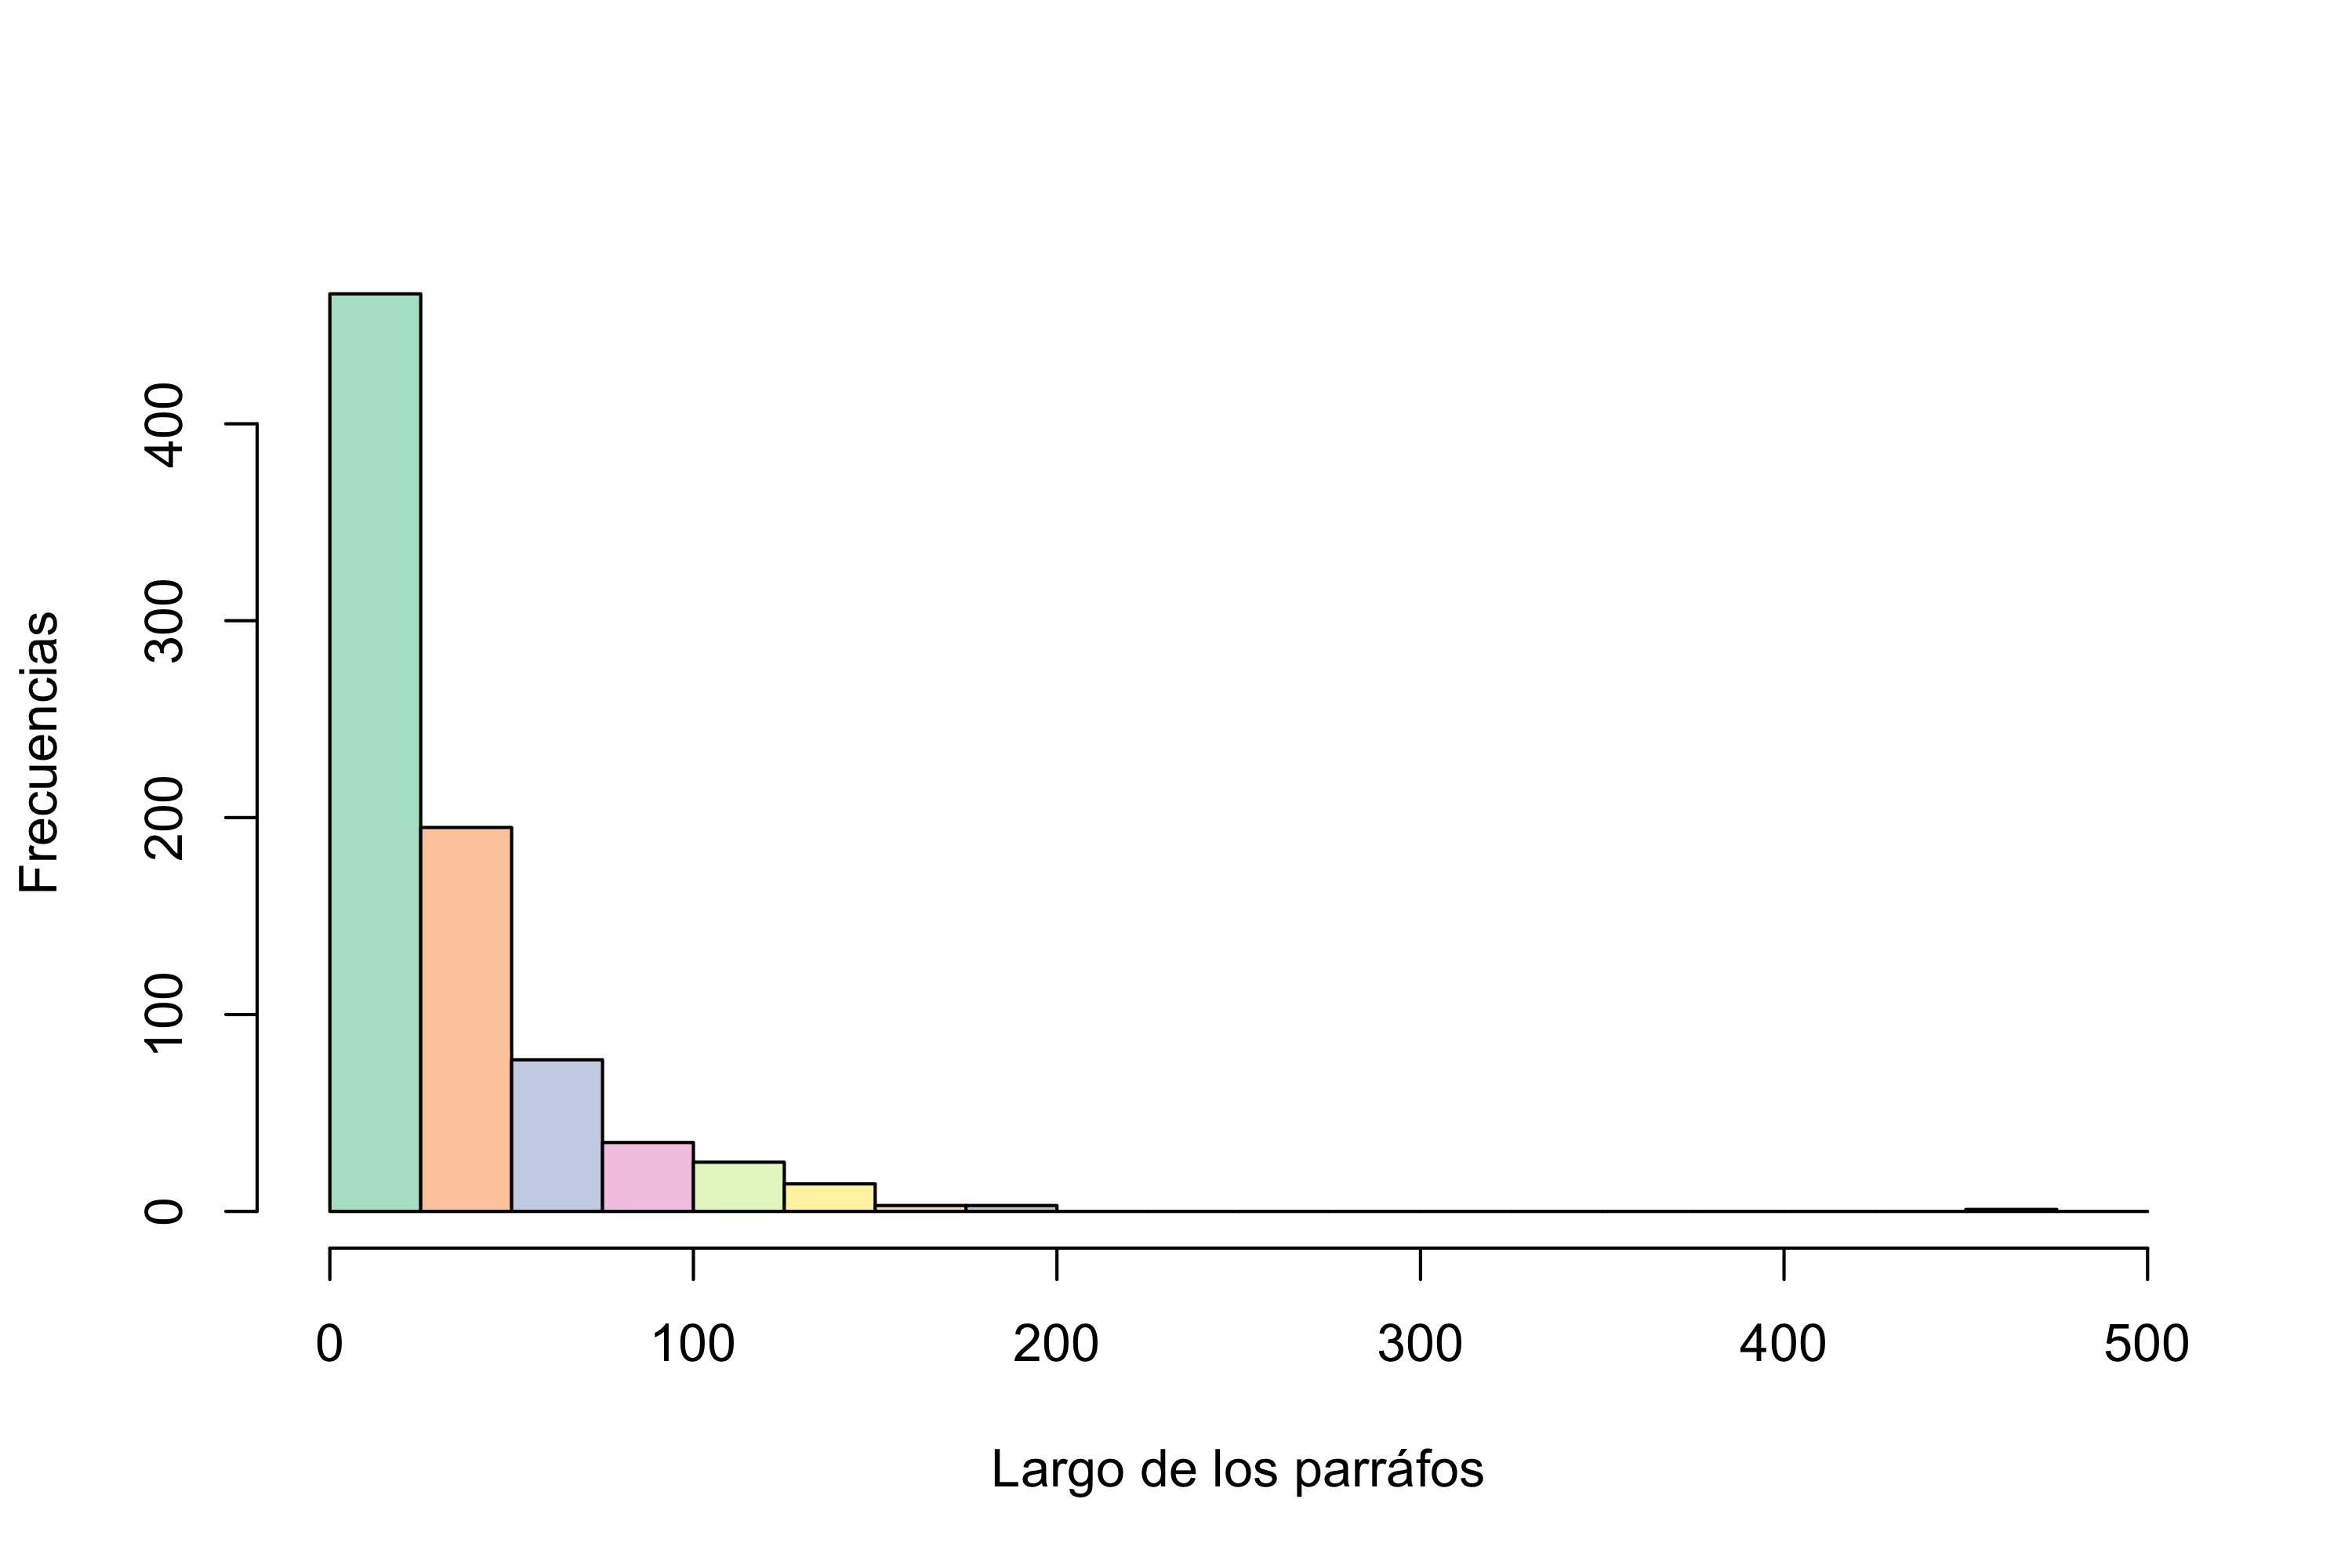
\includegraphics[width=\linewidth]{Largo_parrafos.png} 		
 		\caption{Largo de los párrafos.}
 		 	\label{parrafos}
 	\end{subfigure}
 	\begin{subfigure}[b]{0.45\linewidth}
 		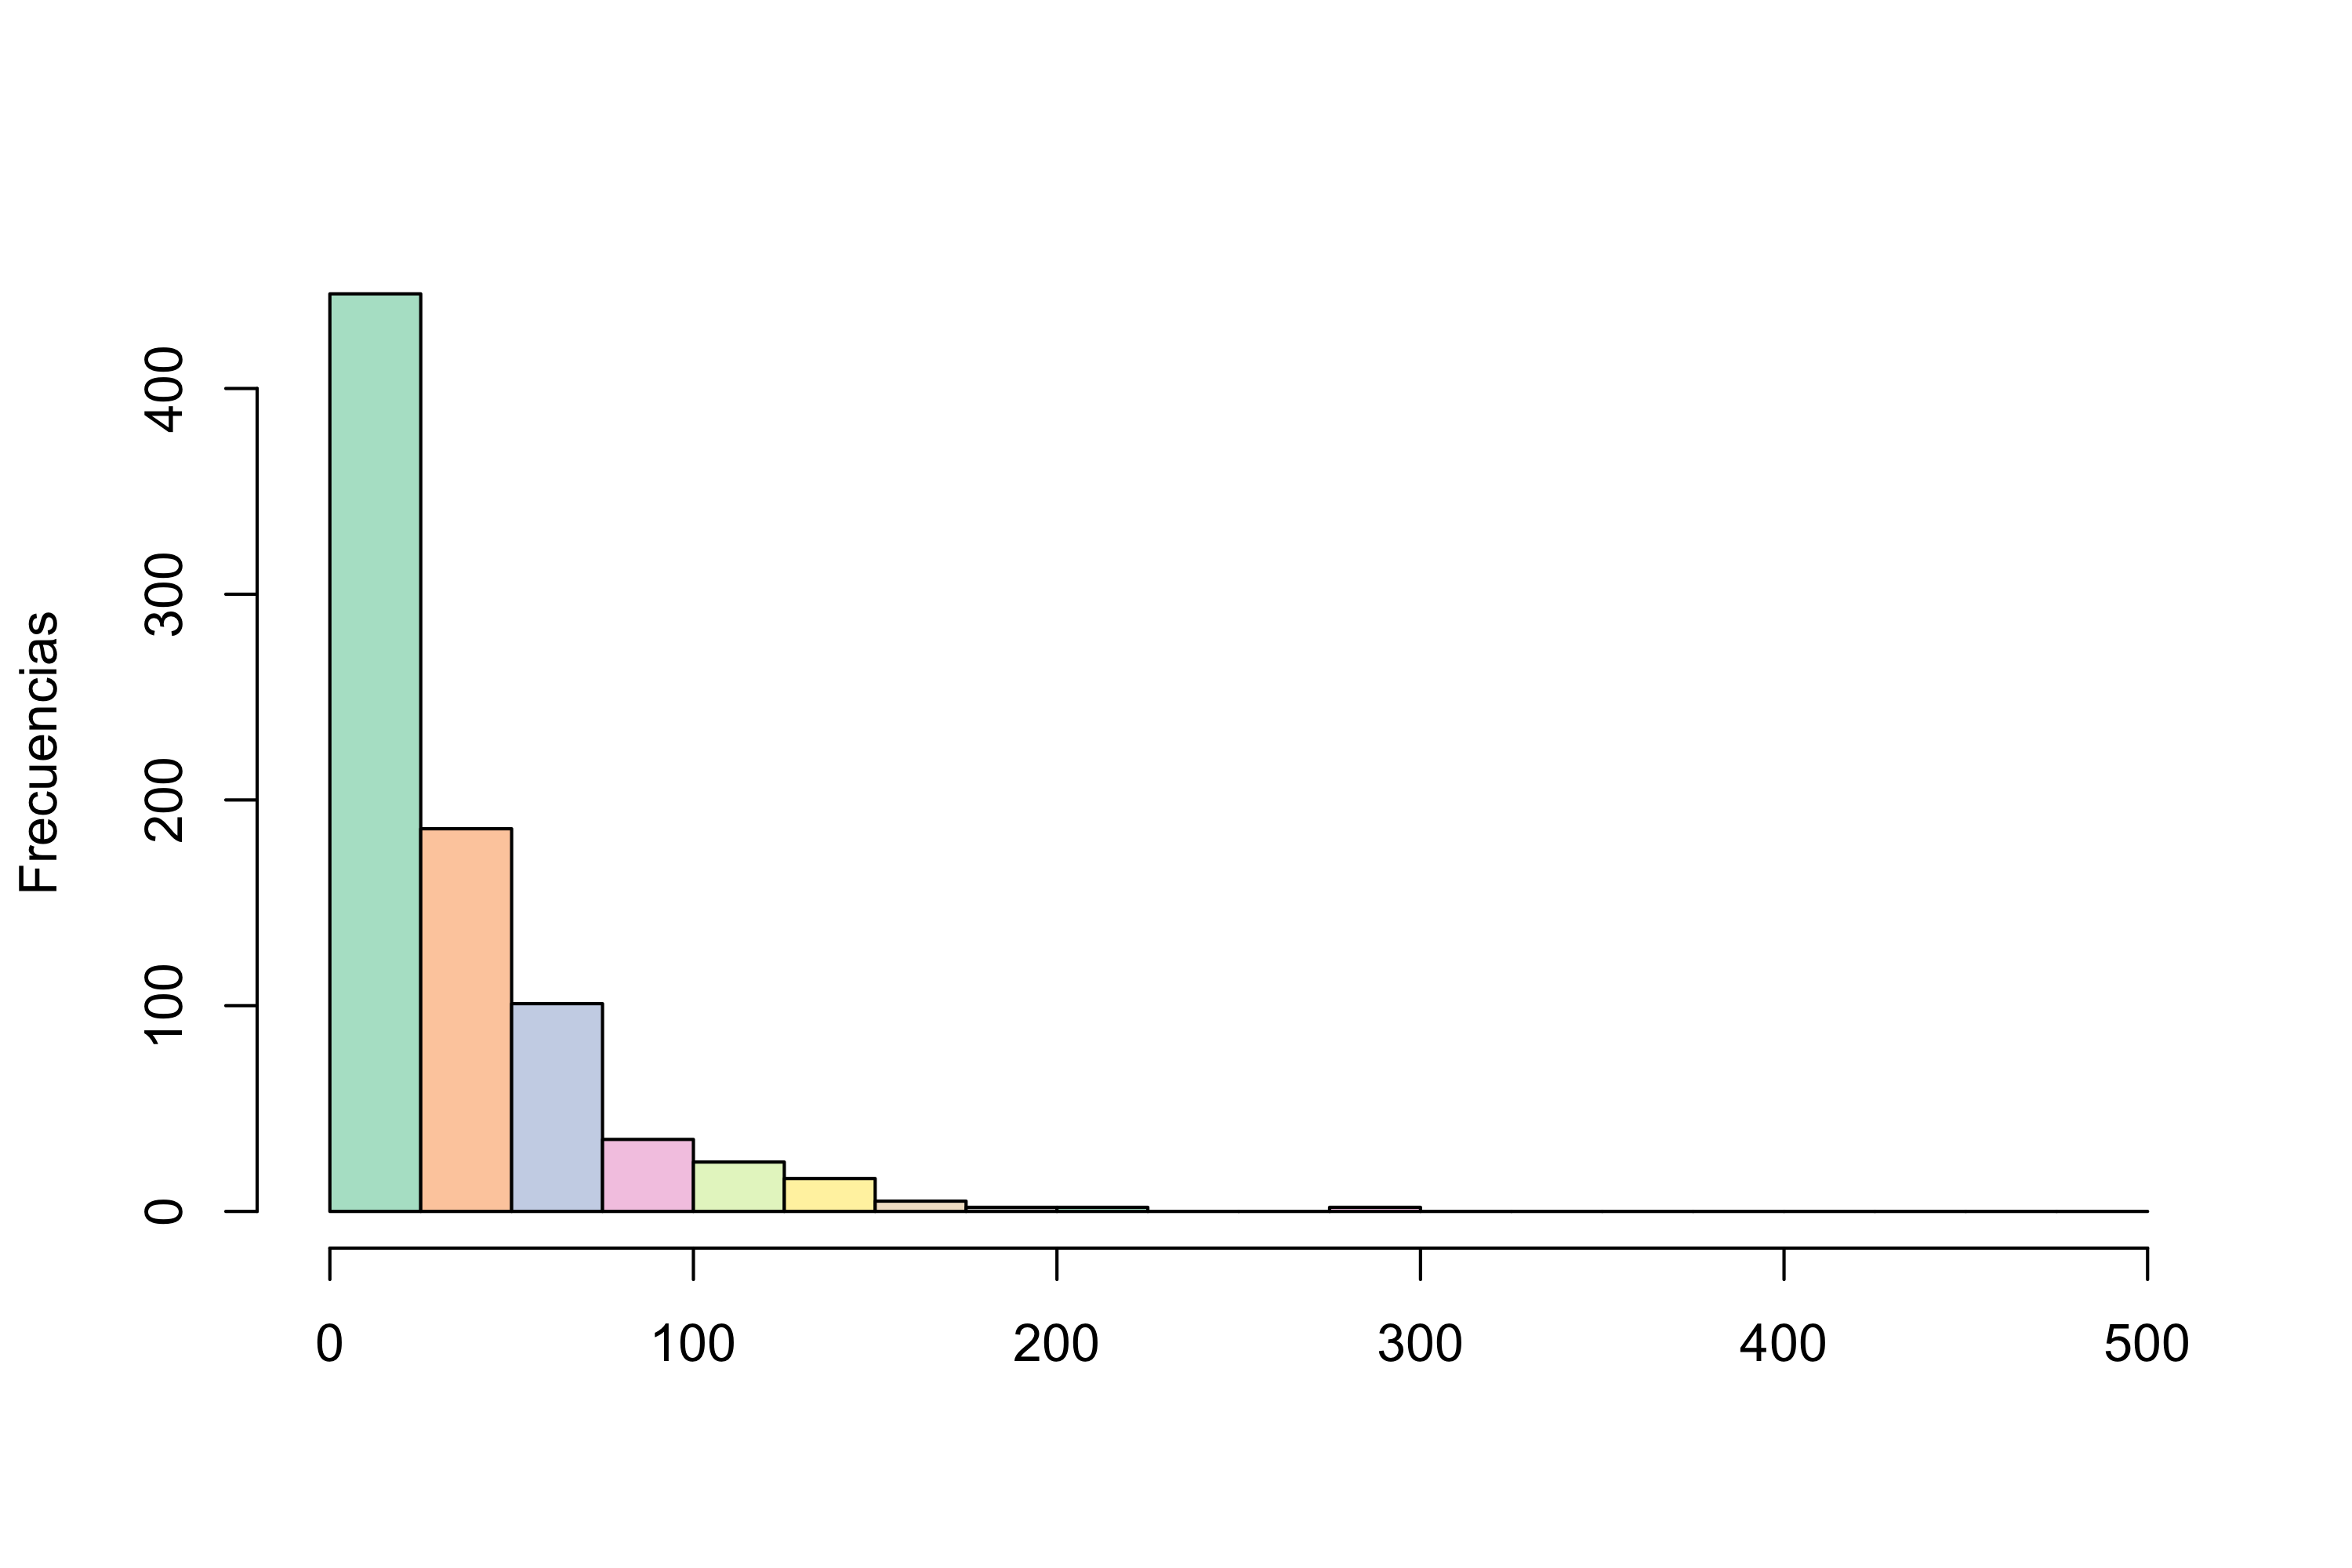
\includegraphics[width=\linewidth]{Largo_parrafos_distribucion.png} 		
 		\caption{Números pseudoaleatorios.}
 		\label{simparrafos}
 	\end{subfigure}
 	 	\caption{Distribución del largo de párrafos.} 
 	 	 	\label{largoparrafos}
\end{figure}




\begin{figure}
 	\centering
 
 	\begin{subfigure}[b]{0.45\linewidth}
 		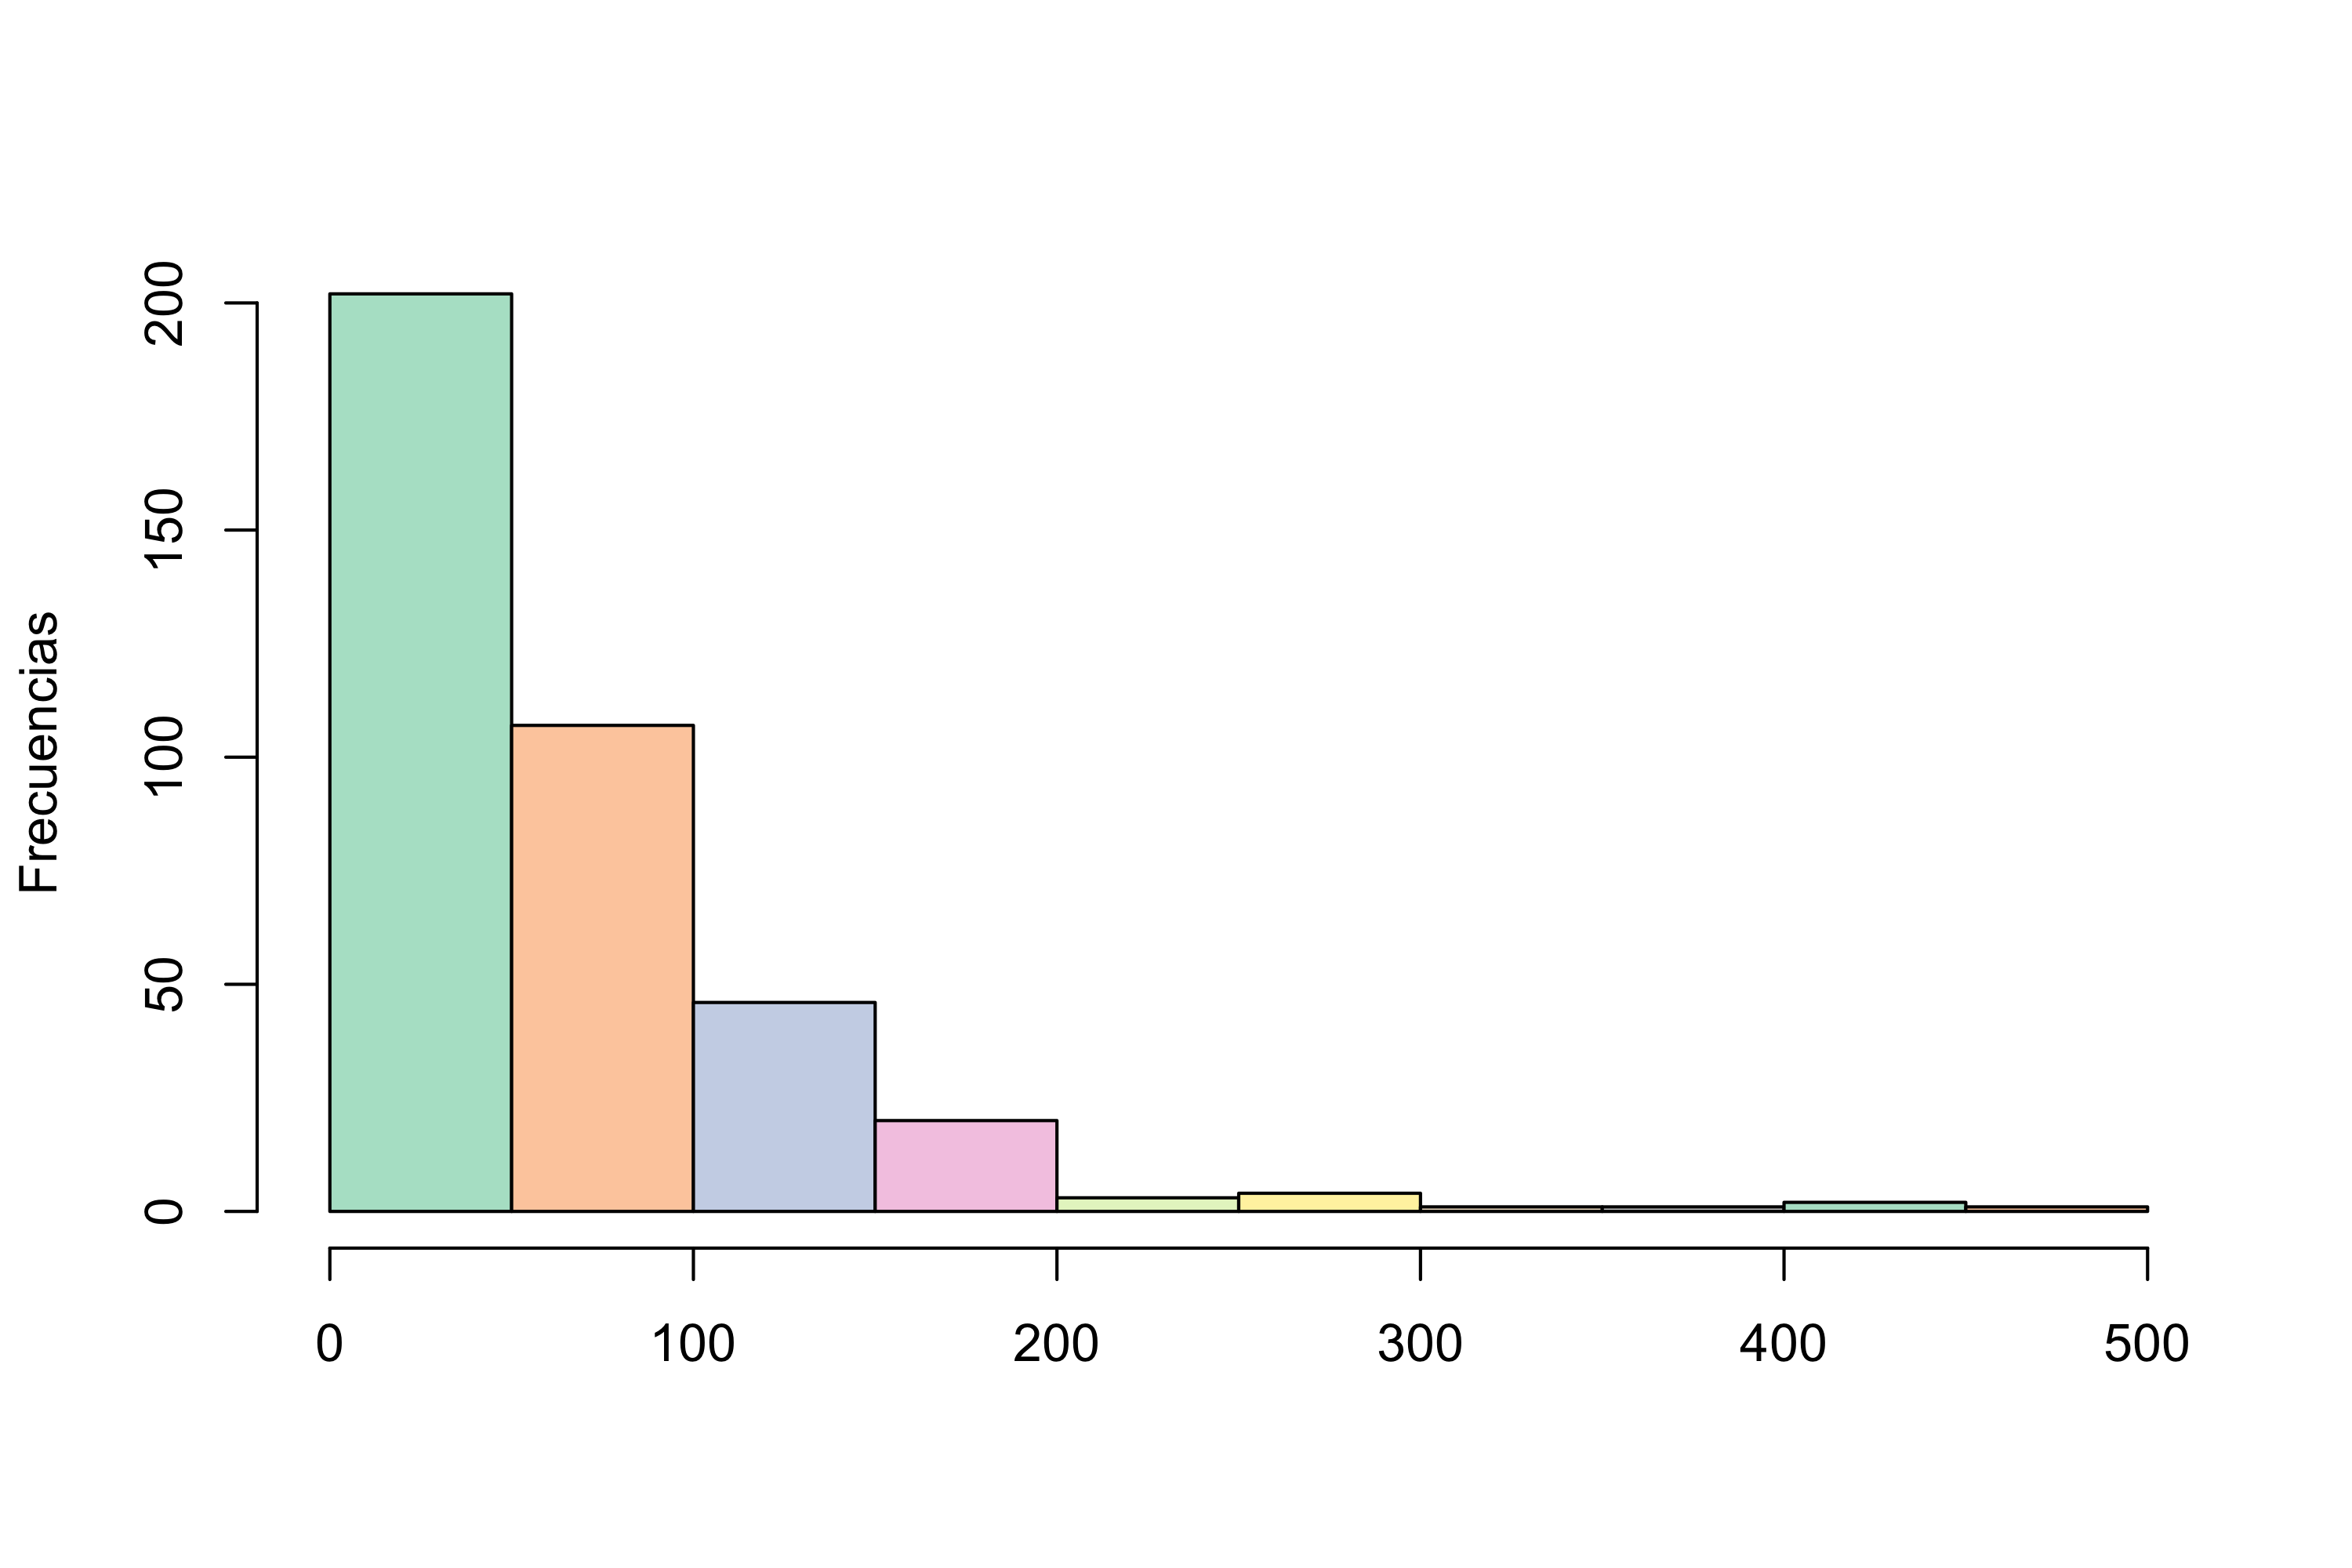
\includegraphics[width=\linewidth]{simulacion.png} 
 		 	\caption{Aparición de la palabra Alice.}
 		 		\label{alice}
 	\end{subfigure}
 	\begin{subfigure}[b]{0.45\linewidth}
 		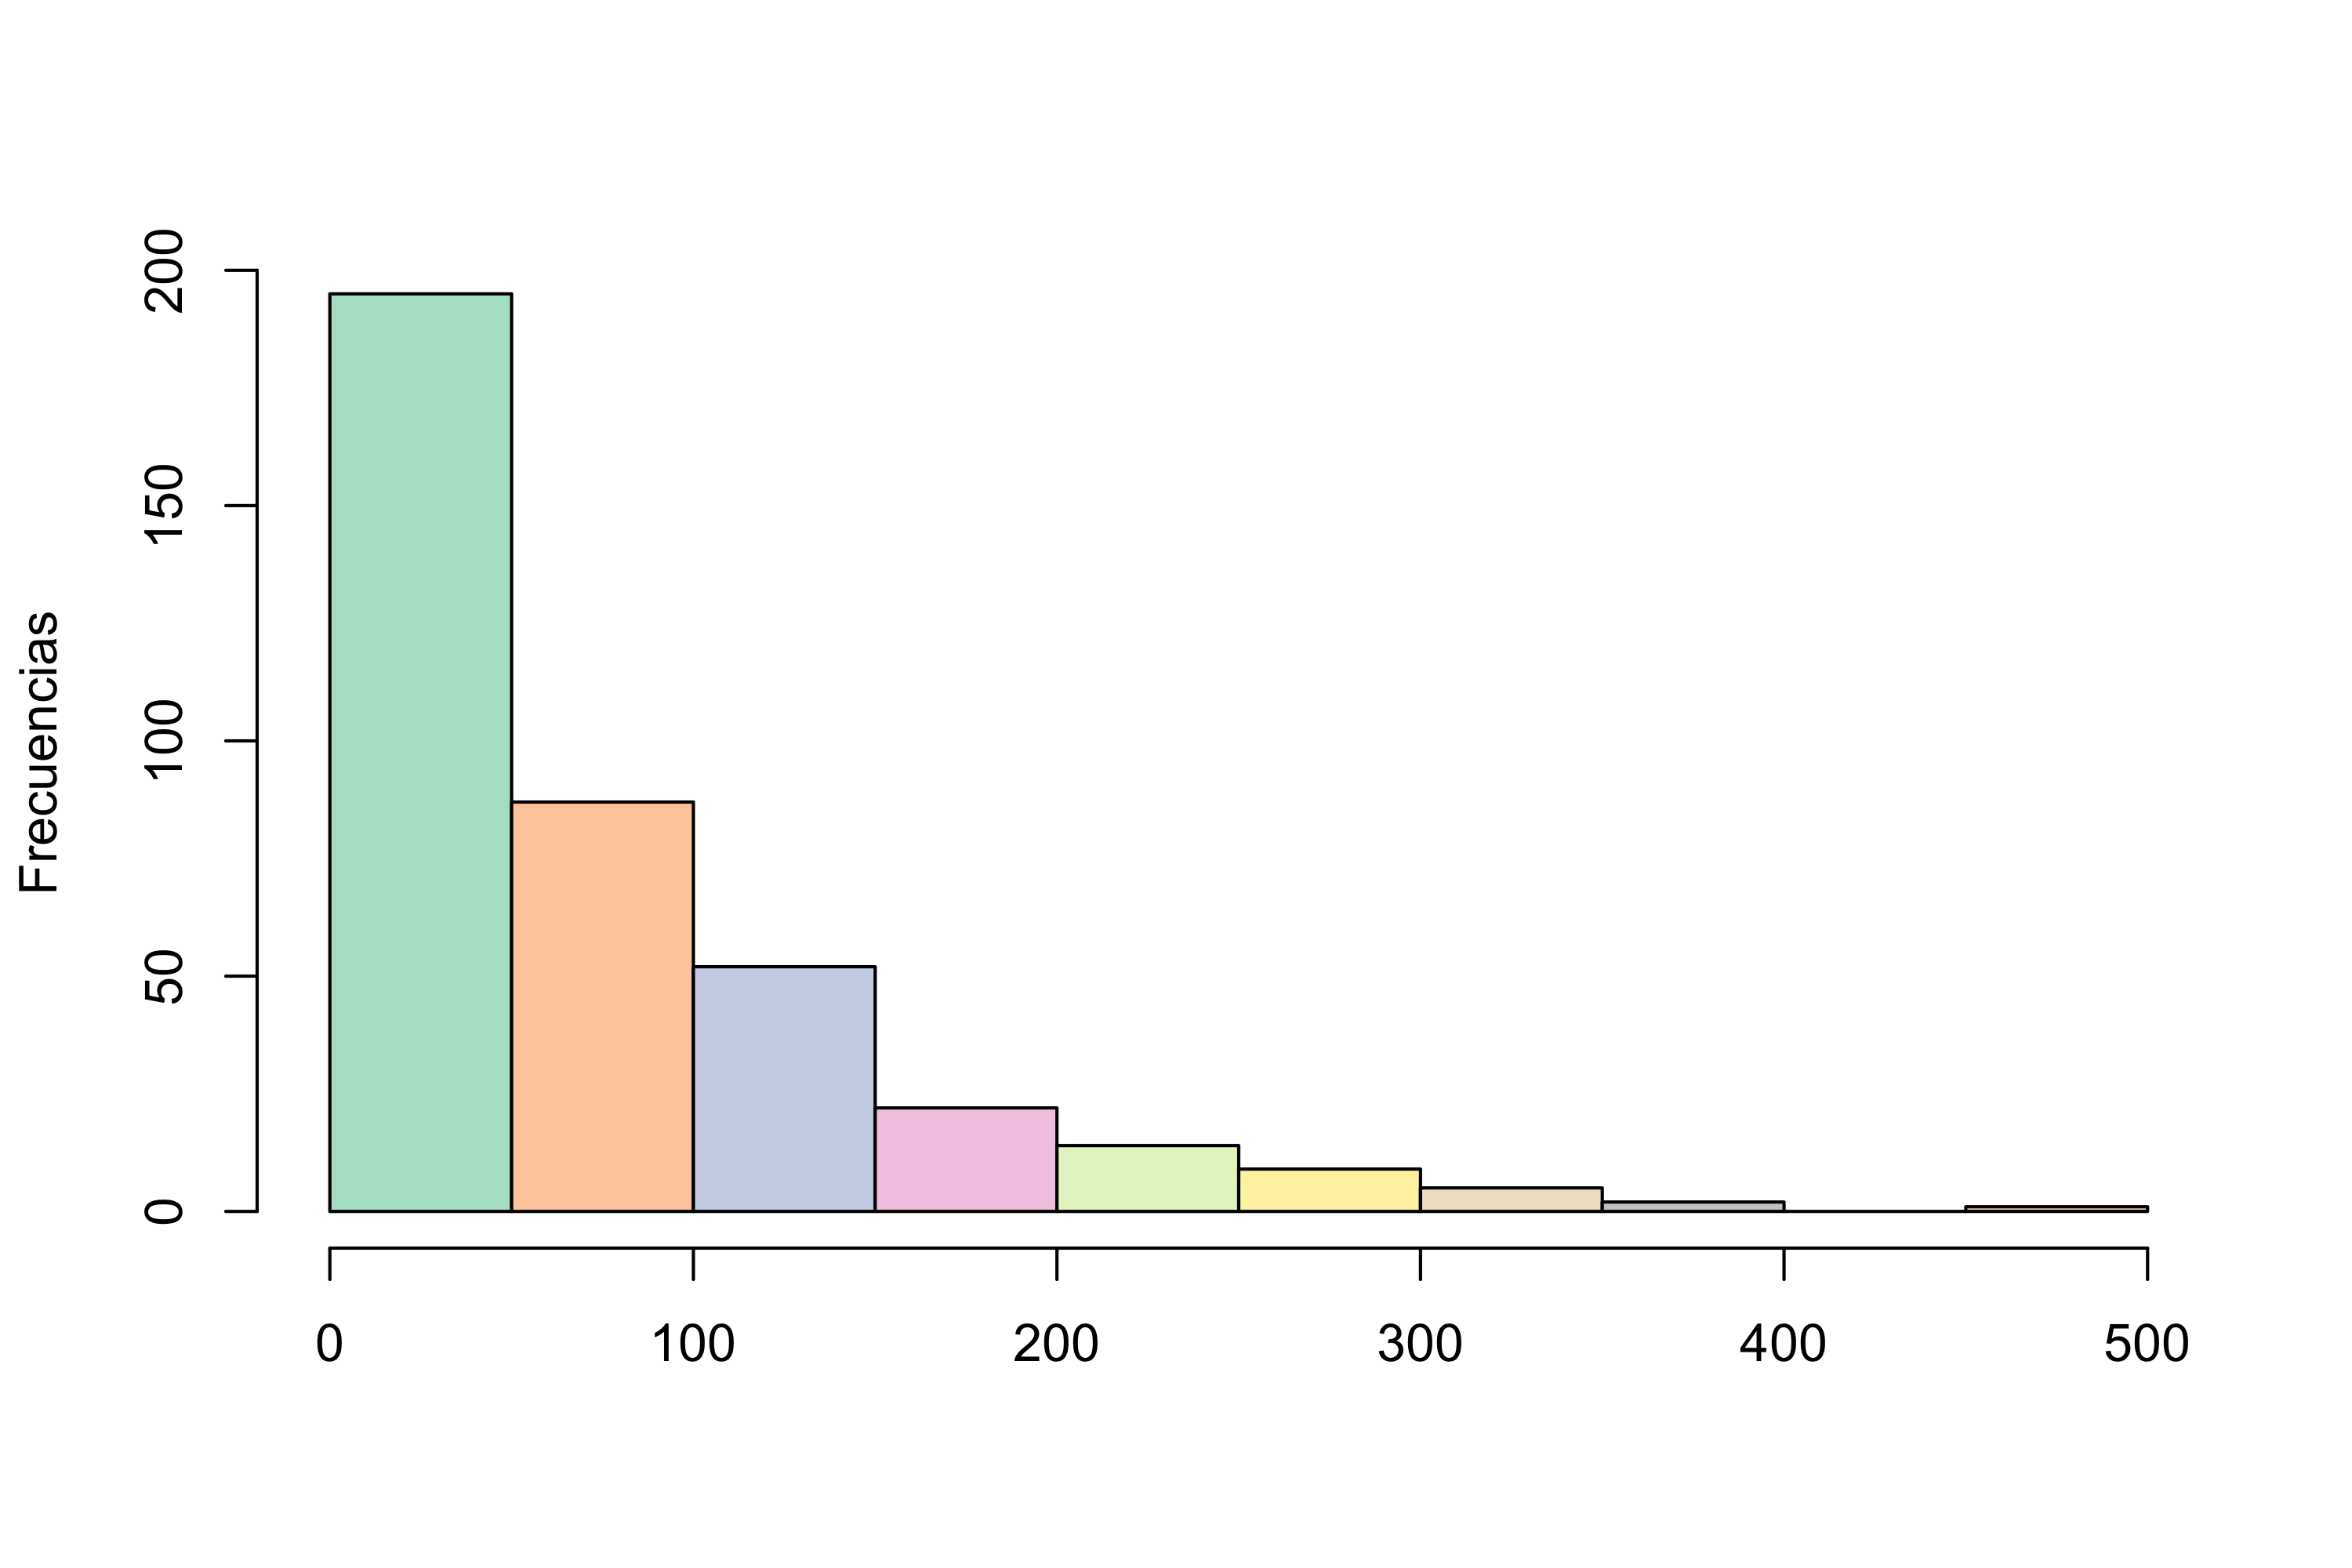
\includegraphics[width=\linewidth]{simulacion_distribucion.png} 		
 		\caption{Números pseudoaleatorios.}
 		\label{simalice}
 	\end{subfigure}
 	 		\label{distAlice}
 	\caption{Distribución de la aparación de la palabra \textit{Alice}.}
\end{figure}


\bibliographystyle{plain} 
\bibliography{Referencias}



\end{document}